\chapter{Specyfikacja techniczna}

\section{Architektura systemu}

W obecnie tworzonych systemach spotyka się dwie podstawowe struktury:
architekturę klient-serwer oraz architekturę trójwarstwową.  W
architekturze klient-serwer, która była szczególnie popularna w latach
dziewięćdziesiątych ubiegłego wieku, wyróżnia się dwie warstwy:
\begin{itemize}
\item aplikację użytkownika (\emph{klient});
\item system zarządzania bazą danych (\emph{serwer}).
\end{itemize}

Struktura ta sprawdza się dla prostych systemów, których zadaniem jest
zapisywanie, odczytywanie oraz aktualizacja danych. Problem pojawia
się jednak w przypadku, gdy dane muszą być przetwarzane w nietrywialny
sposób, przy uwzględnieniu dziedziny problemu (ang. \emph{domain
  logic}) modelowanego zagadnienia. Realizacja obliczeń w warstwie
klienta, której głównym zadaniem jest prezentacja informacji
użytkownikowi, może znacząco wpływać na jego komfort pracy oraz
powodować problemy związane z duplikacją kodu źródłowego aplikacji.
Natomiast umieszczenie logiki aplikacji po stronie serwera bardzo
często narzuca przygotowanie programu w środowisku specyficznym dla
danego systemu zarządzania bazami danych.

Problemy te zmusiły projektantów aplikacji do wydzielenia jeszcze
jednego poziomu, który jest odpowiedzialny za logikę operacji na
danych. W architekturze trójwarstwowej uwzględnione są następujące
warstwy:
\begin{itemize}
\item warstwa prezentacji;
\item warstwa aplikacji;
\item warstwa źródła danych.
\end{itemize}

\begin{figure}[h]
  \begin{center}
    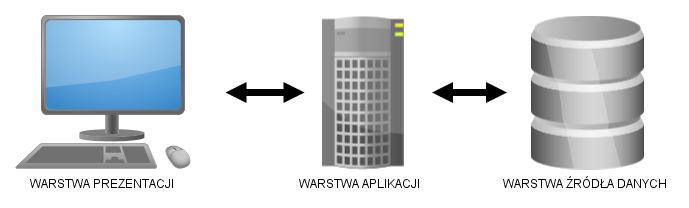
\includegraphics[scale=0.5]{../img/arch-3warstw.png}
  \end{center}
  \label{fig:arch3warstw}
  \caption{Schemat architektury trójwarstwowej}
\end{figure}
\FloatBarrier

W przypadku realizowanego systemu do obsługi magazynu zastosowana
będzie architektura trójwarstwowa.

Na warstwę prezentacji realizowanego systemu składa się:
\begin{itemize}
\item okienkowy interfejs użytkownika (dla kierownika oraz
  magazyniera);
\item serwis webowy (dla sprzedawcy).
\end{itemize}
Warstwa prezentacji komunikuje się z aplikacją w celu wykonania
określonej operacji. Warstwa aplikacji składa się z:
\begin{itemize}
\item warstwy usługowej (serwisów), które są odpowiedzialne za 
  wykonywanie niezbędnych operacji (obliczeń, sprawdzania poprawności
  danych wejściowych itp.);
\item warstwy dostępu do danych (DAO).
\end{itemize}

Podstawę całego systemu stanowi relacyjna baza danych.
Schematy bazy danych opracowany został na podstawie 
modelu analitycznego. Przygotowane zostały również
perspektywy udostępniające aplikacji tylko niezbędne
informacje.

\section{Sprzęt i oprogramowanie}


